% Options for packages loaded elsewhere
\PassOptionsToPackage{unicode=true}{hyperref}
\PassOptionsToPackage{hyphens}{url}
%
\documentclass[
]{article}
\usepackage{lmodern}
\usepackage{amssymb,amsmath}
\usepackage{ifxetex,ifluatex}
\ifnum 0\ifxetex 1\fi\ifluatex 1\fi=0 % if pdftex
  \usepackage[T1]{fontenc}
  \usepackage[utf8]{inputenc}
  \usepackage{textcomp} % provides euro and other symbols
\else % if luatex or xelatex
  \usepackage{unicode-math}
  \defaultfontfeatures{Scale=MatchLowercase}
  \defaultfontfeatures[\rmfamily]{Ligatures=TeX,Scale=1}
\fi
% Use upquote if available, for straight quotes in verbatim environments
\IfFileExists{upquote.sty}{\usepackage{upquote}}{}
\IfFileExists{microtype.sty}{% use microtype if available
  \usepackage[]{microtype}
  \UseMicrotypeSet[protrusion]{basicmath} % disable protrusion for tt fonts
}{}
\makeatletter
\@ifundefined{KOMAClassName}{% if non-KOMA class
  \IfFileExists{parskip.sty}{%
    \usepackage{parskip}
  }{% else
    \setlength{\parindent}{0pt}
    \setlength{\parskip}{6pt plus 2pt minus 1pt}}
}{% if KOMA class
  \KOMAoptions{parskip=half}}
\makeatother
\usepackage{xcolor}
\IfFileExists{xurl.sty}{\usepackage{xurl}}{} % add URL line breaks if available
\IfFileExists{bookmark.sty}{\usepackage{bookmark}}{\usepackage{hyperref}}
\hypersetup{
  pdftitle={STAT 205 HW4},
  pdfauthor={HONGLEI REN},
  hidelinks,
}
\urlstyle{same} % disable monospaced font for URLs
\usepackage[margin=1in]{geometry}
\usepackage{color}
\usepackage{fancyvrb}
\newcommand{\VerbBar}{|}
\newcommand{\VERB}{\Verb[commandchars=\\\{\}]}
\DefineVerbatimEnvironment{Highlighting}{Verbatim}{commandchars=\\\{\}}
% Add ',fontsize=\small' for more characters per line
\usepackage{framed}
\definecolor{shadecolor}{RGB}{248,248,248}
\newenvironment{Shaded}{\begin{snugshade}}{\end{snugshade}}
\newcommand{\AlertTok}[1]{\textcolor[rgb]{0.94,0.16,0.16}{#1}}
\newcommand{\AnnotationTok}[1]{\textcolor[rgb]{0.56,0.35,0.01}{\textbf{\textit{#1}}}}
\newcommand{\AttributeTok}[1]{\textcolor[rgb]{0.77,0.63,0.00}{#1}}
\newcommand{\BaseNTok}[1]{\textcolor[rgb]{0.00,0.00,0.81}{#1}}
\newcommand{\BuiltInTok}[1]{#1}
\newcommand{\CharTok}[1]{\textcolor[rgb]{0.31,0.60,0.02}{#1}}
\newcommand{\CommentTok}[1]{\textcolor[rgb]{0.56,0.35,0.01}{\textit{#1}}}
\newcommand{\CommentVarTok}[1]{\textcolor[rgb]{0.56,0.35,0.01}{\textbf{\textit{#1}}}}
\newcommand{\ConstantTok}[1]{\textcolor[rgb]{0.00,0.00,0.00}{#1}}
\newcommand{\ControlFlowTok}[1]{\textcolor[rgb]{0.13,0.29,0.53}{\textbf{#1}}}
\newcommand{\DataTypeTok}[1]{\textcolor[rgb]{0.13,0.29,0.53}{#1}}
\newcommand{\DecValTok}[1]{\textcolor[rgb]{0.00,0.00,0.81}{#1}}
\newcommand{\DocumentationTok}[1]{\textcolor[rgb]{0.56,0.35,0.01}{\textbf{\textit{#1}}}}
\newcommand{\ErrorTok}[1]{\textcolor[rgb]{0.64,0.00,0.00}{\textbf{#1}}}
\newcommand{\ExtensionTok}[1]{#1}
\newcommand{\FloatTok}[1]{\textcolor[rgb]{0.00,0.00,0.81}{#1}}
\newcommand{\FunctionTok}[1]{\textcolor[rgb]{0.00,0.00,0.00}{#1}}
\newcommand{\ImportTok}[1]{#1}
\newcommand{\InformationTok}[1]{\textcolor[rgb]{0.56,0.35,0.01}{\textbf{\textit{#1}}}}
\newcommand{\KeywordTok}[1]{\textcolor[rgb]{0.13,0.29,0.53}{\textbf{#1}}}
\newcommand{\NormalTok}[1]{#1}
\newcommand{\OperatorTok}[1]{\textcolor[rgb]{0.81,0.36,0.00}{\textbf{#1}}}
\newcommand{\OtherTok}[1]{\textcolor[rgb]{0.56,0.35,0.01}{#1}}
\newcommand{\PreprocessorTok}[1]{\textcolor[rgb]{0.56,0.35,0.01}{\textit{#1}}}
\newcommand{\RegionMarkerTok}[1]{#1}
\newcommand{\SpecialCharTok}[1]{\textcolor[rgb]{0.00,0.00,0.00}{#1}}
\newcommand{\SpecialStringTok}[1]{\textcolor[rgb]{0.31,0.60,0.02}{#1}}
\newcommand{\StringTok}[1]{\textcolor[rgb]{0.31,0.60,0.02}{#1}}
\newcommand{\VariableTok}[1]{\textcolor[rgb]{0.00,0.00,0.00}{#1}}
\newcommand{\VerbatimStringTok}[1]{\textcolor[rgb]{0.31,0.60,0.02}{#1}}
\newcommand{\WarningTok}[1]{\textcolor[rgb]{0.56,0.35,0.01}{\textbf{\textit{#1}}}}
\usepackage{graphicx,grffile}
\makeatletter
\def\maxwidth{\ifdim\Gin@nat@width>\linewidth\linewidth\else\Gin@nat@width\fi}
\def\maxheight{\ifdim\Gin@nat@height>\textheight\textheight\else\Gin@nat@height\fi}
\makeatother
% Scale images if necessary, so that they will not overflow the page
% margins by default, and it is still possible to overwrite the defaults
% using explicit options in \includegraphics[width, height, ...]{}
\setkeys{Gin}{width=\maxwidth,height=\maxheight,keepaspectratio}
\setlength{\emergencystretch}{3em} % prevent overfull lines
\providecommand{\tightlist}{%
  \setlength{\itemsep}{0pt}\setlength{\parskip}{0pt}}
\setcounter{secnumdepth}{-\maxdimen} % remove section numbering
% Redefines (sub)paragraphs to behave more like sections
\ifx\paragraph\undefined\else
  \let\oldparagraph\paragraph
  \renewcommand{\paragraph}[1]{\oldparagraph{#1}\mbox{}}
\fi
\ifx\subparagraph\undefined\else
  \let\oldsubparagraph\subparagraph
  \renewcommand{\subparagraph}[1]{\oldsubparagraph{#1}\mbox{}}
\fi

% Set default figure placement to htbp
\makeatletter
\def\fps@figure{htbp}
\makeatother


\title{STAT 205 HW4}
\author{HONGLEI REN}
\date{03/04/2020}

\begin{document}
\maketitle

\hypertarget{ex-9.21}{%
\section{EX 9.21}\label{ex-9.21}}

\hypertarget{a-an-exploratory-data-analysis.}{%
\subsubsection{(a) An exploratory data
analysis.}\label{a-an-exploratory-data-analysis.}}

\begin{Shaded}
\begin{Highlighting}[]
\NormalTok{  FEVdata <-}\StringTok{ }\KeywordTok{read.table}\NormalTok{(}\DataTypeTok{file=}\StringTok{"FullFEVdata.txt"}\NormalTok{,}\DataTypeTok{header=}\NormalTok{T, }\DataTypeTok{sep=}\StringTok{""}\NormalTok{) }
  \KeywordTok{attach}\NormalTok{(FEVdata)}
  \KeywordTok{pairs}\NormalTok{(}\OperatorTok{~}\NormalTok{Age}\OperatorTok{+}\NormalTok{Hgt}\OperatorTok{+}\NormalTok{Male}\OperatorTok{+}\NormalTok{Smoke}\OperatorTok{+}\NormalTok{FEV,}\DataTypeTok{labels=}\KeywordTok{c}\NormalTok{(}\StringTok{"Age"}\NormalTok{,}\StringTok{"Height"}\NormalTok{,}\StringTok{"Male"}\NormalTok{,}\StringTok{"Smoke"}\NormalTok{,}\StringTok{"FEV"}\NormalTok{),}\DataTypeTok{data=}\NormalTok{FEVdata)}
\end{Highlighting}
\end{Shaded}

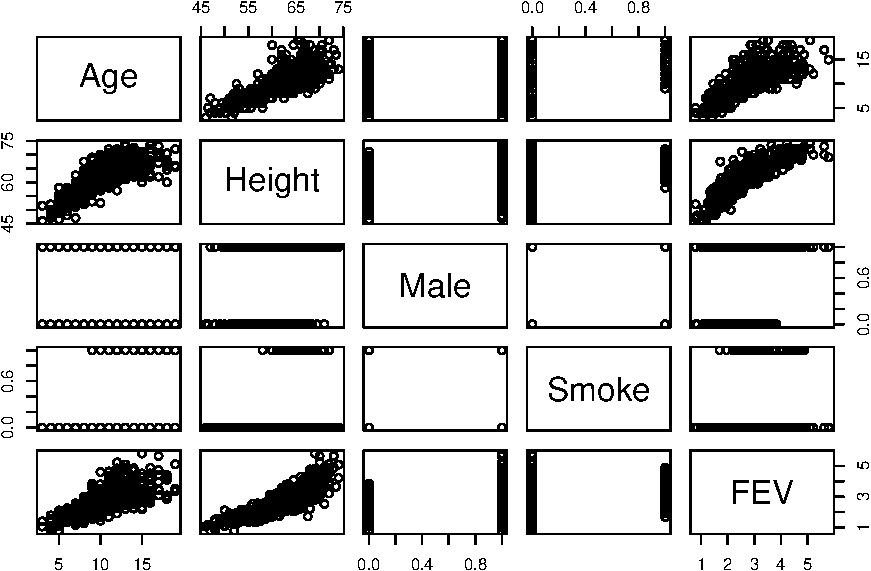
\includegraphics{STAT_205_HW4_files/figure-latex/unnamed-chunk-1-1.pdf}
From the figure above, we can see that Age and Height are postively
correlated and FEV increases as either of them increase.
Smoke-adolescents in this study range from 7 to 18 years old, and have
higher FEV.

\begin{Shaded}
\begin{Highlighting}[]
\NormalTok{  Age.st=}\KeywordTok{standardize}\NormalTok{(Age)}
\NormalTok{  Hgt.st=}\KeywordTok{standardize}\NormalTok{(Hgt)}
\NormalTok{  FEV.st=}\KeywordTok{standardize}\NormalTok{(FEV)}
\NormalTok{  X.mat=}\KeywordTok{model.matrix}\NormalTok{(}\OperatorTok{~}\StringTok{ }\KeywordTok{as.factor}\NormalTok{(Male) }\OperatorTok{+}\StringTok{ }\KeywordTok{as.factor}\NormalTok{(Smoke) }\OperatorTok{+}\StringTok{ }\NormalTok{Age.st }\OperatorTok{+}\StringTok{ }\NormalTok{Hgt.st }\OperatorTok{+}\StringTok{ }\KeywordTok{as.factor}\NormalTok{(Smoke)}\OperatorTok{*}\NormalTok{Age.st }\OperatorTok{+}\StringTok{ }\NormalTok{Age.st }\OperatorTok{*}\StringTok{ }\NormalTok{Hgt.st)}
\end{Highlighting}
\end{Shaded}

\end{document}
